%%%%%%%%%%%%%%%%%%%%%%%%%%%%%%%%%%%%%%%%%%%%%%%%%%%%%%%%%%%%%%%%%
% Contents : The entrance chapter
% $Id : grisbi-manuel-entrance.tex, v 2.0 2021/mm/dd Jean-Luc Duflot
%%%%%%%%%%%%%%%%%%%%%%%%%%%%%%%%%%%%%%%%%%%%%%%%%%%%%%%%%%%%%%%%%

\chapter{Entrée dans Grisbi\label{entrance}}

Au démarrage de l'application, Grisbi affiche sa page 
\ifIllustration d'entrée\refimage{entrance-img}. Si ce n'est pas le cas, vous pouvez afficher la fenêtre de Grisbi en \indexword{plein écran}\index{affichage !plein écran}\index{plein écran !affichage} par la touche de fonction \key{F11}, et revenir en arrière par la même touche.
\else d'entrée. Si ce n'est pas le cas, vous pouvez afficher la fenêtre de Grisbi en \indexword{plein écran}\index{affichage !plein écran}\index{plein écran !affichage} par la touche de fonction \key{F11}, et revenir en arrière par la même touche.
\fi

% espace   : 5 mm
%\vspacepdf{5mm}

%Cette page vous permet de démarrer Grisbi de différentes manières.


%Vous pouvez afficher la fenêtre de Grisbi en \indexword{plein écran}\index{affichage !plein écran}\index{plein écran !affichage} par la touche de fonction \key{F11}, et revenir en arrière par la même touche.

\ifIllustration
% image centrée
\begin{figure}[htbp]
\begin{center}
\includegraphics[scale=0.35]{image/screenshot/entrance}
\end{center}
\caption{Entrée dans Grisbi}
\label{entrance-img}
\end{figure}
% image centrée
\fi

%% espace   : 5 mm
%\vspacepdf{5mm}
%\ifIllustration
%% image centrée
%\begin{figure}[htbp]
%	\begin{center}
%		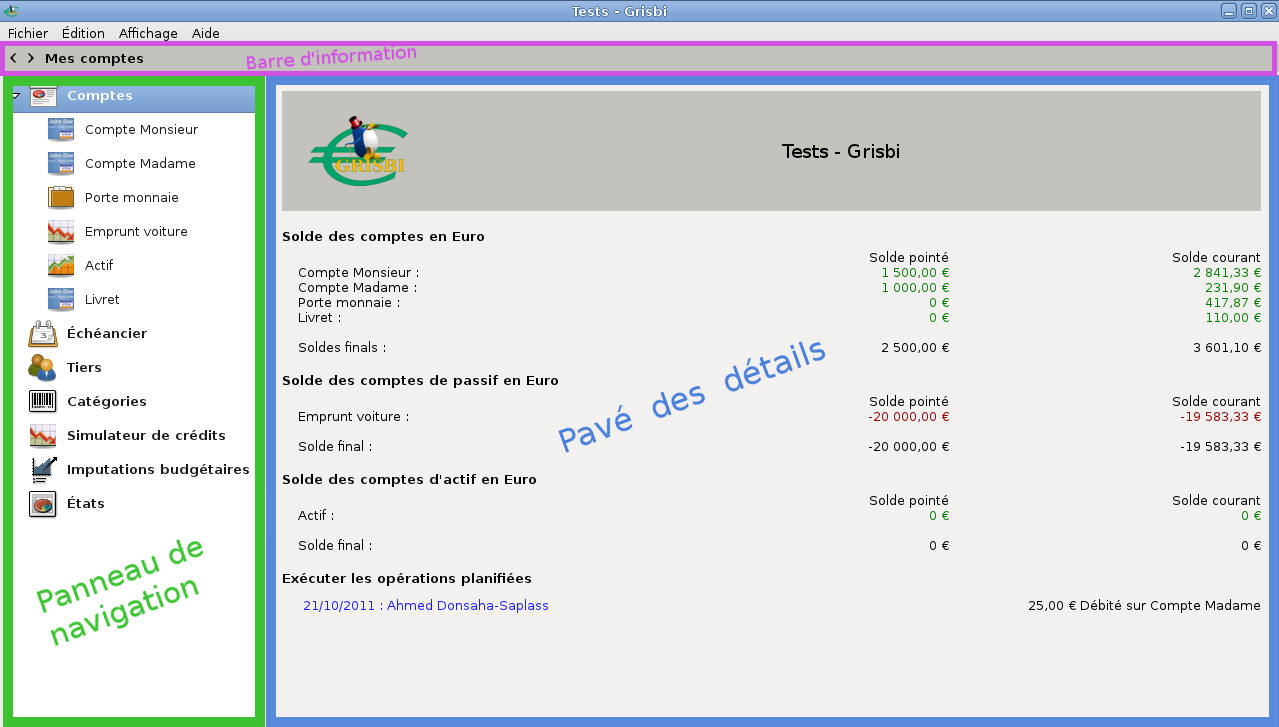
\includegraphics[scale=0.35]{image/screenshot/home}
%	\end{center}
%	\caption{Page d'accueil}
%	\label{home-img}
%\end{figure}
%% image centrée
%\fi

Cette page affiche plusieurs pavés ;

\begin{itemize}
	 \item le pavé Nouveau, pour lancer l'assistant d'Aide à la création d'un nouveau fichier de comptes ;
	 \item le pavé Ouvrir, pour afficher un gestionnaire de fichier avec lequel vous pourrez chercher un fichier de comptes existant dans votre ordinateur ;
	 \item le pavé Importer, pour lancer l'assistant d'Aide à l'importation de fichiers ;
	 \item un ou plusieurs autres pavés, portant le nom de fichiers de comptes, si Grisbi en a déjà ouvert ; si vous voulez les enlever de cette page d'entrée, déplacez les fichiers dans un autre répertoire, ou supprimez-les.
\end{itemize}

% espace   : 5 mm
%\vspacepdf{5mm}

%\textbf{Note} : les pavés portant les noms des fichiers de compte que Grisbi a déjà utilisés ne sont présents que si ces fichiers existent ; si vous voulez les enlever de cette page d'entrée, déplacez les dans un autre répertoire, ou supprimez-les.

% espace   : 5 mm
%\vspacepdf{5mm}



% espace   : 5 mm
\vspacepdf{5mm}

En bas de page, un bandeau vous appelle à choisir une action, en sélectionnant l'un de ces pavés. Si vous voulez juste découvrir le logiciel Grisbi pour avoir un aperçu de son aspect et de ses possibilités, vous pouvez à la place utiliser un fichier exemple (voir la section \vref{new-example}, \menu{Fichier Exemple}).
















